\documentclass[10pt]{beamer}

\usepackage[english]{babel}
\usepackage[utf8]{inputenc}
\usepackage{hyperref}
\usepackage{verbatim}
\usepackage{multicol}

\newcommand{\code}[1]{\texttt{#1}}
\newcommand{\outline}[0]{
  \frame{\frametitle{Outline}\tableofcontents[hideallsubsections]}
}
\newcommand{\outlinereminder}[0]{
  \frame{\frametitle{Outline}
  \tableofcontents[currentsection,subsectionstyle=show/show/hide]}
}


%      _         _             _                     _                     
%  ___| |_ _   _| | ___    ___| |_    ___ ___  _   _| | ___ _   _ _ __ ___ 
% / __| __| | | | |/ _ \  / _ \ __|  / __/ _ \| | | | |/ _ \ | | | '__/ __|
% \__ \ |_| |_| | |  __/ |  __/ |_  | (_| (_) | |_| | |  __/ |_| | |  \__ \
% |___/\__|\__, |_|\___|  \___|\__|  \___\___/ \__,_|_|\___|\__,_|_|  |___/
%          |___/                                                           
%

\setbeamercovered{transparent}
\usetheme{Warsaw}
% enlever [red] dans le \documentclass si utilisation de la suite :
\usecolortheme[RGB={202,31,39}]{structure} % rouge

%\setbeamertemplate{background}{\includegraphics[height=96mm,width=128mm]{fond.png}}

% definition de la couleur du fond des blocks
\definecolor{ArrierePlanBodyW}{rgb}{0.5,0.5,0.5} % si ecriture blanche
\definecolor{ArrierePlanBodyB}{rgb}{0.9,0.9,0.9} % si ecriture noire
% definition de la couleur des slides
\definecolor{ArrierePlan}{rgb}{1,1,1}

\definecolor{darkred}{rgb}{0.6,0,0}

\definecolor{toutnoir}{rgb}{0,0,0}

% selection de la couleur du fond des slides
\setbeamercolor{background canvas}{bg=ArrierePlan} 
% selection de la couleur du fond des block avec ecriture noire
\setbeamercolor{block body}{use=structure,fg=black,bg=ArrierePlanBodyB}
% selection de la couleur du fond des block avec ecriture blanche
%\setbeamercolor{block body}{use=structure,fg=white,bg=ArrierePlanBodyW}

%\setbeamercolor{section in head/foot}{toutnoir}

\setbeamertemplate{footline}{%
  \leavevmode%
  \hbox{\begin{beamercolorbox}[wd=.5\paperwidth,ht=2.5ex,dp=1.125ex,leftskip=.3cm plus1fill,rightskip=.3cm]{author in head/foot}%
    \usebeamerfont{author in head/foot}\insertshortauthor
  \end{beamercolorbox}%
  \begin{beamercolorbox}[wd=.5\paperwidth,ht=2.5ex,dp=1.125ex,leftskip=.3cm,rightskip=.3cm plus1fil]{title in head/foot}%
    \usebeamerfont{title in head/foot}\insertshorttitle \hfill \insertframenumber{} / \inserttotalframenumber\hspace*{2ex}%
  \end{beamercolorbox}}%
  \vskip0pt%
}


\setbeamercovered{dynamic}
%\logo{\includegraphics[height=1cm]{./img/logo_petit-tr.png}}
% \defbeamertemplate*{headline}{split theme}
% {%
%   \begin{beamercolorbox}{section in head/foot}
%     \insertsectionnavigationhorizontal{2cm}{\includegraphics[height=2cm]{./img/logo_petit-tr.png}}{}
%   \end{beamercolorbox}%
%  }

\defbeamertemplate*{headline}{}
{%
%   \begin{beamercolorbox}[wd=.1\paperwidth,ht=\tempdimb]{section in head/foot}
%      \vbox to 1cm{\vfil\includegraphics[.1\paperwidth]{./img/logo_petit-tr.png}\vfil}%
%   \end{beamercolorbox}
  \leavevmode%
  \begin{beamercolorbox}[wd=.095\paperwidth,ht=1.45cm]{section in head/foot}%
    \vbox to 1.45cm{\vfill\hspace*{1mm}
\includegraphics[height=1.25cm]{lifc.png}\vfill}%
  \end{beamercolorbox}%
  \begin{beamercolorbox}[wd=.405\paperwidth,ht=1.45cm]{section in head/foot}%
    \vbox to 1.45cm{\vfil\insertsectionnavigation{.4\paperwidth}\vfil}%
  \end{beamercolorbox}%
  \begin{beamercolorbox}[wd=.33\paperwidth,ht=1.45cm]{subsection in head/foot}%
    \vbox to 1.45cm{\vfil\insertsubsectionnavigation{.4\paperwidth}\vfil}%
  \end{beamercolorbox}%
  \begin{beamercolorbox}[wd=.17\paperwidth,ht=1.45cm]{section in head/foot}%
%     \vbox to 1.5cm{\vfil
\includegraphics[width=.145\paperwidth]{./img/ufc2.pdf}\vfill}%
%      \vbox to 1.5cm{\vfill
\includegraphics[width=.185\paperwidth]{./img/ufc2.pdf}\vfill}%
      \vbox to 1.45cm{\vfill\hspace*{-0.1mm}
\includegraphics[height=1.45cm]{ufc2.pdf}\vfill}%
  \end{beamercolorbox}%
}



\title[Praspel: Contract-Driven Testing for PHP]{Praspel: A Specification Language for Contract-Driven Testing in PHP}
\author{
    \textbf{Ivan~Enderlin} \and
    Frédéric~Dadeau \and
    Alain~Giorgetti \and
    Abdallah~Ben~Othman
}
\date{
    November 9th, 2011 \\
    ICTSS, Paris
}


\begin{document}

\maketitle

\begin{frame}
\frametitle{Motivations}

\begin{block}{Context}
\begin{itemize}
\item Types are the main verification mechanism massively adopted
\item Annotation is more and more a common processus for developers
\item Unit testing is used to maintain large softwares (with a thousand of
manual tests)
\end{itemize}
\end{block}

\begin{block}{Initial ideas}
\begin{itemize}
\item An easy language to express contracts
\item Automate tests (data) generation and execution
\item A complete, clean and modular test framework
\end{itemize}
\end{block}

\end{frame}

\begin{frame}
\frametitle{Design-by-Contract}

\begin{block}{Definition}
\begin{itemize}
\item Invented by B. Meyer in 1992 with Eiffel language
\item Describes a model using annotations
\item Expresses formal constraints: pre-, postconditions, invariants…
\item Included directly in the source code: classes attributes, methods
arguments…
\end{itemize}
\end{block}

\begin{block}{Semantics of contracts}
\begin{itemize}
\item Contractual agreement:
  \begin{itemize}
  \item caller: “I commit to satisfy your pre-condition when I'm calling you”
  \item called: “In this case, I commit to establish my post-condition”
  \end{itemize}
\item Invariants must be satisfied before and after the execution of the methods
\end{itemize}
\end{block}

\end{frame}

\begin{frame}
\frametitle{Design-by-Contract}

\begin{block}{Existing contract-based specification languages}
\begin{itemize}
\item Spec\#: for C\# language, contracts are written in C\#
\item JML: Java Modeling Language, contracts are expressed with logic formulæ
\item ACSL: ANSI/C Specification Language, adds algebraic structures
\item Nothing for PHP
\end{itemize}
\end{block}
Initially designed for verification (static or dynamic)

\end{frame}

\begin{frame}
\frametitle{Contract-Driven Testing}

\begin{block}{Definition}
Exploits the contract for generating tests:
\begin{itemize}
\item uses preconditions to generate test data
\item uses postconditions to establish test verdict by runtime assertion
checking
\end{itemize}
\end{block}

\begin{block}{Issue}
\begin{itemize}
\item How to describe realistic data for being able to generate them?
\end{itemize}
\end{block}

\end{frame}

\begin{frame}
\frametitle{Contributions}

\begin{itemize}
\item Realistic domains
  \begin{itemize}
  \item overlay/refinement of types
  \item structures to automate the validation and the generation for test data
  \end{itemize}
\item Praspel, a new specification language
  \begin{itemize}
  \item adopts Design-by-Contract paradigm
  \item based on realistic domains
  \item implementation in PHP for PHP
  \end{itemize}
\item Automated unit test generator
  \begin{itemize}
  \item uses Praspel to perform Contract-Driven Testing
  \end{itemize}
\end{itemize}

\end{frame}

\outline

\section{Realistic domains for PHP}

\begin{frame}
\frametitle{About of realistic domains}

\begin{block}{Definition and goal}
\begin{itemize}
\item Specify a set of relevant values that can be assigned to a data for a
specific context (e.g. an email address) in a given program
\item Come with properties for the validation and generation of data values
\item Realistic domains are intended to be used for test generation purposes
\end{itemize}
\end{block}

\begin{block}{Two important properties}
\begin{itemize}
\item \textbf{Predicability}, checks if a value belongs to the realistic domain
\item \textbf{Samplability}, generates values that belong to the realistic
domain; the sampler can be of many kinds: a random generator, a walk in the
domain, an incrementation of values etc.
\end{itemize}
Properties are implemented by the end-user.
\end{block}

\end{frame}

\begin{frame}[fragile]
\frametitle{Realistic domains in PHP}

\begin{block}{Implementation}
In PHP, we have implemented realistic domains as classes providing at least two
methods, corresponding to the two features of realistic domains:
\begin{itemize}
\item \code{predicate(\$q)}, takes a value \code{\$q} as input, returns a
boolean indicating the membership of the value to the realistic domain
\item \code{sample(\$sampler)}, generates values that belong to the realistic
domain according to a basic numeric-sampler \code{\$sampler}
\end{itemize}
\end{block}

\begin{exampleblock}{Skeleton of a realistic domain}
{
\tiny
\begin{verbatim}
class MyOwnRealdom extends ... {

    public function predicate ( $q               ) { return $aBoolean = ...; }
    public function sample    ( Sampler $sampler ) { return $data     = ...; }
}
\end{verbatim}
}
\end{exampleblock}

\end{frame}

\begin{frame}
\frametitle{Hierarchy}

Our implementation exploits the PHP object programming paradigm:
\begin{block}{Hierarchical inheritance}
PHP realistic domains can inherit from each other
\begin{center}
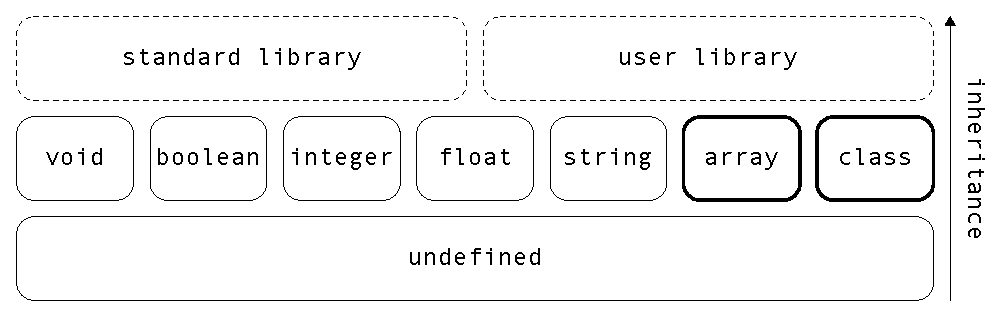
\includegraphics[width=8cm]{Figures/Realdom_univers.pdf}
\end{center}
\end{block}

\begin{block}{What does it imply?}

The predicate of a child realistic domain can refine its parent predicate by
adding new constraints. Default sampler: parent sampler and rejection.

\end{block}

\end{frame}

\begin{frame}
\frametitle{Parameters}

\begin{block}{Parameterizable}
Realistic domains may have parameters. They can receive arguments of many kinds:
constants or realistic domains themselves
\end{block}

\begin{exampleblock}{Basic realistic domain with constant arguments}
\code{boundinteger(7, 42)} contains all the integers between 7 and 42
\end{exampleblock}

% simplifier
\begin{exampleblock}{Realistic domain with constants and realistic domains as
arguments}
\code{string(boundinteger(4, 12), 0x20, 0x7e)} is intended to contain all
the strings of length between 4 and 12 constitued of characters from \code{0x20}
to \code{0x7e} (Unicode code-points)
\end{exampleblock}

\begin{exampleblock}{User-defined realistic domain}
\code{email()} is intended to contain all email addresses
% ça, c'est à transposer en version code (figures de l'adresse email);
\end{exampleblock}

\end{frame}

\section{Implementation in Praspel}

\outlinereminder

\begin{frame}
\frametitle{Presentation of Praspel}

\begin{block}{Signification and format}
\begin{itemize}
\item PHP Realistic Annotation and SPEcification Language
\item Written in the API documentation (\code{/** ... */})
\item Makes it possible to express formal constraints, called {\em clauses}
(starting with the standard \code{@} symbol)
\end{itemize}
\end{block}

\end{frame}

\subsection{Assigning realistic domains to data}

\begin{frame}
\frametitle{Operator \code{:}}

\begin{block}{Syntax and semantics}
The syntactic construction:
\begin{center}
\code{$i$: $t_1$(\dots) or \dots~or $t_n$(\dots)}
\end{center}
associates at least one realistic domain among $t_1$(\dots), \dots,
$t_n$(\dots) to an identifier $i$.
\end{block}

\begin{exampleblock}{Examples of realistic domains declarations}
\begin{itemize}
\item \code{y: integer() or float() or boolean()} means that \code{y} can
either be an integer, a floating-point number or a boolean
\item \code{u: email() or userLogin()} specifies that \code{u} is either an
email address or a user login
\end{itemize}
\end{exampleblock}

\end{frame}

\begin{frame}
\frametitle{Array description}

\begin{block}{Syntax and semantics}
An array {\em description} has the following form:
\begin{center}
\begin{tabular}{llllll}
  \code{array([} &
  \code{from} &
  \code{$T^1_1$(\dots)} &
  \code{or \dots~or} &
  \code{$T^1_i$(\dots)} \\
  &
  \code{to} &
  \code{$T^1_{i+1}$(\dots)} &
  \code{or \dots~or} &
  \code{$T^1_n$(\dots),} \\
  &
  \code{\vdots} \\
  &
  \code{from} &
  \code{$T^k_1$(\dots)} &
  \code{or \dots~or} &
  \code{$T^k_j$(\dots)} \\
  &
  \code{to} &
  \code{$T^k_{j+1}$(\dots)} &
  \code{or \dots~or} &
  \code{$T^k_m$(\dots)} &
  \code{], $size$)}
\end{tabular}
\end{center}
\code{from} {\em domains} \code{to} {\em co-domains} ({\em pairs} separated by
\code{,}), each ones are domains disjunctions.
\end{block}

\end{frame}

\begin{frame}
\frametitle{Array description}

\begin{exampleblock}{Examples of arrays}
\begin{itemize}
\item \code{a$_1$: array([from integer() to boolean(), boundinteger(7, 42))}
\item \code{a$_2$: array([to boolean(), to float()], 7)}
\item \code{a$_3$: array([to boolean() or float()], 7)}
\item \code{a$_4$: array([to integer()], boundinteger(1, 256))}
\end{itemize}
\end{exampleblock}

\end{frame}

\subsection{Designing contracts in Praspel}

\begin{frame}
\frametitle{Defining a contract clause}

\begin{block}{Contract content}
\begin{itemize}
\item either the assignment of a realistic domain to a given data (\code{:})
\item or it is a predicate $\backslash$\code{pred(…) }(expressed in the PHP
syntax)
\item enriched with the $\backslash$\code{result} and
$\backslash$\code{old($e$)} constructs
\end{itemize}
\end{block}

\begin{block}{Praspel clauses}
Applied on classes:
\begin{itemize}
\item \code{@invariant}, invariant on class attributes
\end{itemize}
Applied on methods:
\begin{itemize}
\item \code{@requires}, precondition on class attributes and method arguments
\item \code{@ensures}, postcondition on class attributes, and method arguments
and result
\item \code{@throwable}, list of throwable exceptions by the method
\end{itemize}
\end{block}

\end{frame}

\begin{frame}[fragile]
\frametitle{Praspel clauses}

\begin{exampleblock}{Example of a short Praspel contract}
{
\scriptsize
\begin{verbatim}
/**
 * @requires needle:   integer() and
 *           haystack: array([to integer()], boundinteger(1, 256)) and
 *           matches:  undefined();
 * @ensures  \result:  boolean() and
 *           matches:  undefined();
 */
public function exists ( $needle,  $haystack, &$matches = false ) {

    $intersect = array_intersect($haystack, array($needle));

    if(null === $matches)
        $matches = array_keys($intersect);

    return 0 < count($intersect);
}
\end{verbatim}
}
\end{exampleblock}

\end{frame}

\begin{frame}[fragile]
\frametitle{Organization in behaviors}

\begin{block}{Several behaviors per method}
\begin{itemize}
\item Each \code{@behavior} clause has a unique name inside a contract
\item A behavioral clause contains \code{@requires}, \code{@ensures} and
\code{@throwable} clauses
\item By default, a global implicit behavior exists
\end{itemize}
\end{block}

\begin{exampleblock}{\code{matches} is no longer \code{undefined}}
{
\scriptsize
\begin{verbatim}
/**
 * @behavior get_matches {
 *     @requires matches: void();
 *     @ensures  matches: array(
 *                            [to boundinteger(0, 255)],
 *                            boundinteger(0, 256)
 *                        );
 * }
 */
\end{verbatim}
}
\end{exampleblock}

\end{frame}

\section{Automated unit test generator}

\outlinereminder

\begin{frame}
\frametitle{Unit test generator and test verdict}

\begin{block}{Contract-Driven Testing}
The testing process works with the two features provided by the realistic
domains:
\begin{itemize}
\item ({\em samplability}) the sampler is implemented as a random data generator
that satisfies the precondition of the method
\item ({\em predicability}) the predicate makes it possible to check the
postcondition at runtime after the execution of the method
\end{itemize}
\end{block}

\begin{overprint}
\onslide<1>
\begin{block}{Random test data generation}
\begin{itemize}
\item Test data generation are used in the \code{sample()} method
\item $\backslash$\code{pred} thus introduces rejection in precondition
\item Random generation was a first approach
\end{itemize}
\end{block}

\onslide<2>
\begin{block}{Runtime Assertion Checking and test verdict}
\begin{itemize}
\item The RAC is performed by instrumenting the initial PHP code with additional
code that checks the contract clauses
\item Detected failures can be of five kinds: precondition, postcondition,
throwable, invariant or internal precondition (propagation) failure
\end{itemize}
\end{block}
\end{overprint}

\end{frame}

\begin{frame}[fragile]
\frametitle{Example of instrumentation}

\begin{exampleblock}{Instrument \code{foo()}}
\begin{multicols}{2}
{
\tiny
\begin{verbatim}
public function foo ( ... ) {

    $this->foo_contract();
    $this->foo_pre(...);

    try {

        $result = $this->foo_body();
    }
    catch ( \Exception $e ) {

        $this->foo_exception($e);
        throw $e;
    }

    $this->foo_post($result, ...);

    return $result;
}
\end{verbatim}
\columnbreak
\begin{verbatim}
public function foo_pre ( ... ) {

    // ...
    return    $contract->verifyInvariants(...)
           && $contract->verifyPreCondition(...);
}

public function foo_post ( $result, ... ) {

    // ...
    return    $contract->verifyPostCondition(
                  $result, ...
              )
           && $contract->verifyInvariants(...);
}

public function foo_exception ( $exception ) {

    return    $contract->verifyException($exception)
           && $contract->verifyInvariants(...);
}
\end{verbatim}
}
\end{multicols}
\end{exampleblock}

\end{frame}

\begin{frame}
\frametitle{Implementation in the Praspel tool}

\begin{block}{Environment for unit testing}
\begin{itemize}
\item Clean and modular framework for generating and executing online tests
\item Praspel and its tools are freely available in Hoa
(\url{http://hoa-project.net}), a set of libraries for PHP
\end{itemize}
\end{block}

\end{frame}

\section{Experimentation}

\outlinereminder

\begin{frame}
\frametitle{Experimentation}

\begin{block}{Case study}
Validate HTML code produced by second year student programs written in PHP, with
different granularities:
\begin{itemize}
\item firstly with a general oracle: is the HTML markup well-formed?
\item secondly with a refined oracle: do attributes exist, are they
well-positionned and are the values right?
\end{itemize}
\end{block}

\begin{block}{Grammar as a dedicated realistic domain}
\begin{itemize}
\item Grammars can be used to validate or generate data
\item It is a new realistic domain
\item Then, we have written a grammar of HTML for the first oracle
\end{itemize}
\end{block}

\end{frame}

\begin{frame}{Observations}

\begin{block}{Simple and easy}
\begin{itemize}
% on a un truc facile à utiliser machin
% on est capable de trouver des erreurs relativement fines : spécifier
% facilement que tel attribut a bien telle valeur liée à un des paramètres
% facile à exprimer et automatiquement vérifier lors de l'exécution
% vachement pratique
\item Experimentation shows that tools are easy to use (2 commands), find bugs
quickly and easily
\item Simple mechanism to describe an oracle
\item Simple mechanism to develop a new realistic domain (here, for grammar)
\item It offers a good ratio effort/results (bugs found)
\end{itemize}
\end{block}

\end{frame}

\section{Conclusion}

\outlinereminder

\begin{frame}
\frametitle{What we have seen?}

\begin{itemize}
\item Realistic domains specifying test data for program variables
  \begin{itemize}
  \item provide two useful features for automated test generation: {\em
  predicability} and {\em samplability}
  \item related work: UDITA has the same approach
  \end{itemize}
\item Praspel, a new Design-by-Contract language implementing realistic domains
\item A test generation and execution framework to automate unit testing in PHP
\item Presently, standard library of 31 realistic domains in Hoa (\code{date},
\code{timestamp}, \code{regex}, \code{bag}, …)
\item We have introduced Grammar-based Testing into a realistic domain
\end{itemize}

\end{frame}

\begin{frame}
\frametitle{Future works}

\begin{itemize}
\item Extend and generalize the concept of realistic domains to other
programming languages to illustrate the benefits of this concept
\item Improve data generators (Search-based Testing, Constraint-based Testing
etc.)
\item Extending standard library of realistic domains
\item[$\star$] Fill the box!
\end{itemize}

\end{frame}

\begin{frame}
\frametitle{Thanks!}

\begin{center}
Thank you for your attention! Any questions?
\end{center}

\end{frame}

\end{document}
